% LaTeX Template for short student reports.
% Citations should be in bibtex format and go in references.bib
\documentclass[a4paper, 11pt]{article}
\usepackage[T1]{fontenc} % font
\usepackage{polski}
\usepackage[utf8]{inputenc}
\usepackage[top=3cm, bottom=3cm, left = 2cm, right = 2cm]{geometry} 
\geometry{a4paper} 
\usepackage[utf8]{inputenc}
\usepackage{textcomp}
\usepackage{graphicx} 
\usepackage{amsmath,amssymb}
\usepackage{booktabs}
\usepackage{bm}  
\usepackage[pdftex,bookmarks,colorlinks,breaklinks]{hyperref}  
\hypersetup{linkcolor=blue,citecolor=blue,filecolor=blue,urlcolor=blue} % black links, for printed output
\usepackage{memhfixc} 
\usepackage{pdfsync}  
\usepackage{fancyhdr}
\pagestyle{fancy}

\title{Lab04}
\author{Max Stróżyk}
%\date{}

\begin{document}
\maketitle
\tableofcontents
\begin{center}
    \href{https://github.com/maxi7524/numerical-methods}{\textbf{Link do projektu na GitHubie}}
\end{center}


\section{Zadanie 1}

\subsection{Charakterystyka metody Hornera}

Metoda Hornera jest techniką stosowaną do szybkiego obliczania wartości wielomianu \( P(x) \) w zadanym punkcie \( x \). Główną zaletą tej metody jest redukcja liczby operacji wymaganych do obliczenia wartości wielomianu, co zmniejsza złożoność obliczeniową z \( O(n^2) \) do \( O(n) \), gdzie \( n \) oznacza stopień wielomianu.

Podstawową ideę algorytmu można przedstawić w następującej formie rekurencyjnej:
\[
P(x) = a_n + x(a_{n-1} + x(a_{n-2} + \dots + x(a_1 + x a_0)))
\]
Dzięki temu każda operacja wymaga jedynie \( n \) mnożeń i \( n \) dodawań, co znacząco zmniejsza czas obliczeń dla dużych stopni wielomianów.

W przeprowadzonych testach dla wielomianów o rozmiarach od 100 do 5000, z krokiem 100, losowano 100 różnych wielomianów dla każdego stopnia. Dla każdego wielomianu mierzono czas obliczenia jego wartości metodą Hornera i standardową, a następnie obliczano średnią z uzyskanych czasów.

\subsection{Wyniki i wnioski}

Poniżej przedstawiono dwa typy wykresów które się pojawiały ilustrujące wyniki eksperymentów:

\begin{center}
\begin{minipage}{0.45\textwidth}
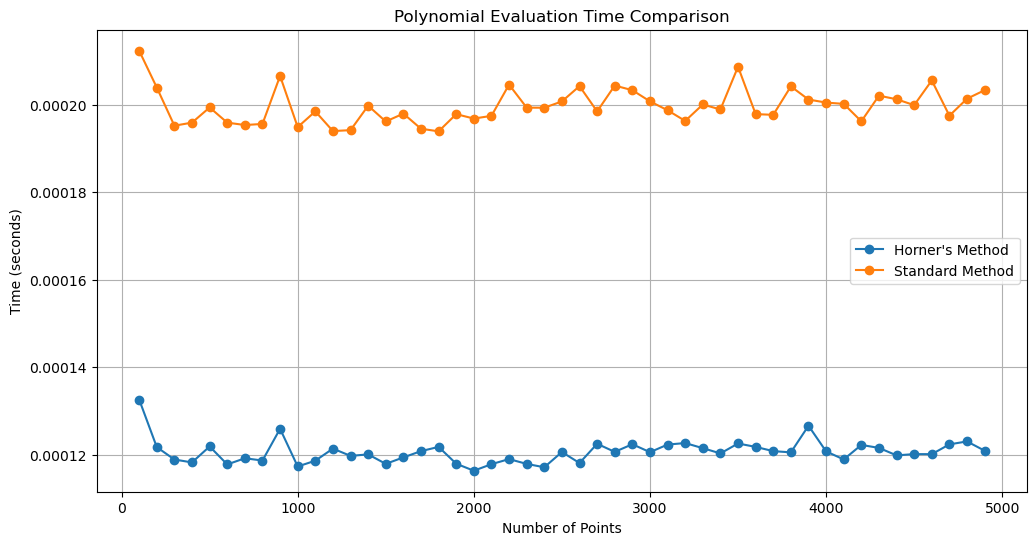
\includegraphics[width=\textwidth]{wykresy/zadanie 1/horner_1.png}
\end{minipage}
\begin{minipage}{0.45\textwidth}
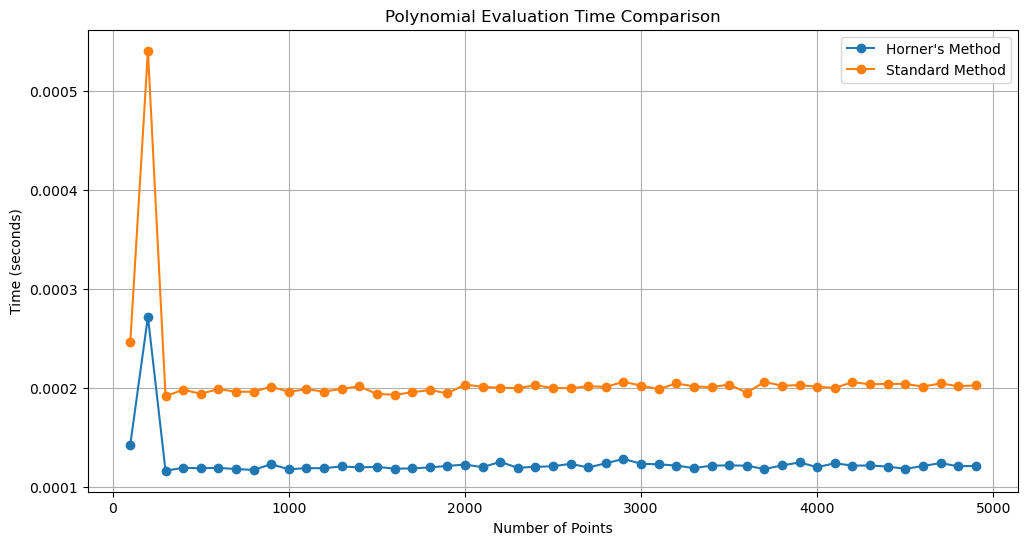
\includegraphics[width=\textwidth]{wykresy/zadanie 1/horner_2.png}
\end{minipage}
\end{center}

\textbf{Wnioski:}
\begin{itemize}
    \item \textbf{Poprawa szybkości algorytmu:} Metoda Hornera pozwala na uzyskanie średniej poprawy szybkości obliczeń na poziomie \( 1.64 \pm 0.04 \). Jest to zgodne z oczekiwaniami wynikającymi ze zmniejszonej złożoności obliczeniowej.
    \item \textbf{Nieoczekiwane skoki czasów:} W niektórych próbach zaobserwowano znaczny wzrost czasu obliczeń dla pojedynczego wielomianu. Zjawisko to nie koreluje z rzędem współczynników ani rozmiarem wielomianu, a jego przyczyna nie jest znana.
    \item \textbf{Skalowalność:} Metoda Hornera wykazuje dobrą skalowalność dla dużych stopni wielomianów, utrzymując stabilny czas obliczeń w porównaniu do klasycznego algorytmu.
\end{itemize}


\newpage



\section{Zadanie 2}

\subsection{Charakterystyka algorytmu Neville'a}

Algorytm Neville'a to metoda numeryczna służąca do wyznaczania wartości interpolowanego wielomianu w danym punkcie. Główną zaletą tej techniki jest możliwość efektywnego obliczania wartości wielomianów na podstawie zadanego zestawu punktów, choć jej złożoność obliczeniowa wynosi \( O(n^2) \), co może być kosztowne przy dużych zbiorach danych.

Interpolacja w algorytmie Neville'a bazuje na rekurencyjnym wzorze, który pozwala obliczyć wartość funkcji w punkcie \( x \) na podstawie danych punktów \( (x_i, y_i) \). Testy przeprowadzono, losując \( n \) punktów z ustalonego przedziału \( D = (0, 10) \), a następnie porównując wartości interpolacji z rzeczywistymi wartościami funkcji w 100 równomiernie rozłożonych punktach.

Eksperyment wykonano dla czterech funkcji:
\begin{itemize}
    \item Funkcja trygonometryczna: \( f(x) = \sin(x) + \cos(x) \),
    \item Wielomian 3 stopnia: \( f(x) = x^3 - 2x + 1 \),
    \item Funkcja wykładnicza: \( f(x) = e^x \),
    \item Funkcja wymierna: \( f(x) = \frac{1}{1 + x^2} \).
\end{itemize}

Dla każdej funkcji obliczono błąd interpolacji oraz odchylenie standardowe, a także czas wywołania algorytmu.

\subsection{Wyniki i wnioski}

% trygonometryczne
\begin{center}
\textbf{Wyniki dla funkcji trygonometrycznej:}  
Najmnieszy błąd: \( 2.01 \times 10^{-13} \pm 1.03 \times 10^{-12} \)  przy 23 punktach  

\begin{minipage}{0.49\textwidth}
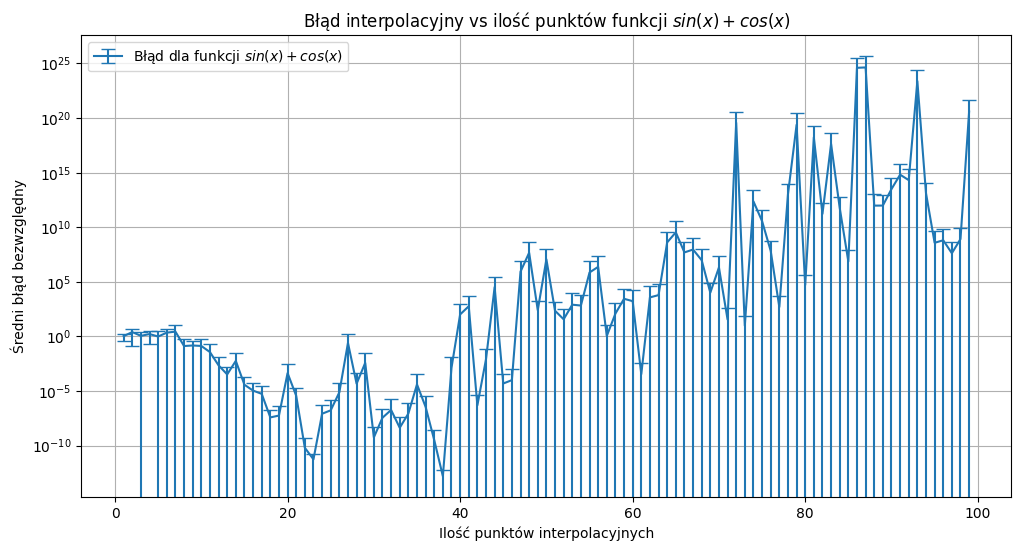
\includegraphics[width=\textwidth]{wykresy/zadanie 2/blad_tryg.png}
\end{minipage}
\begin{minipage}{0.49\textwidth}
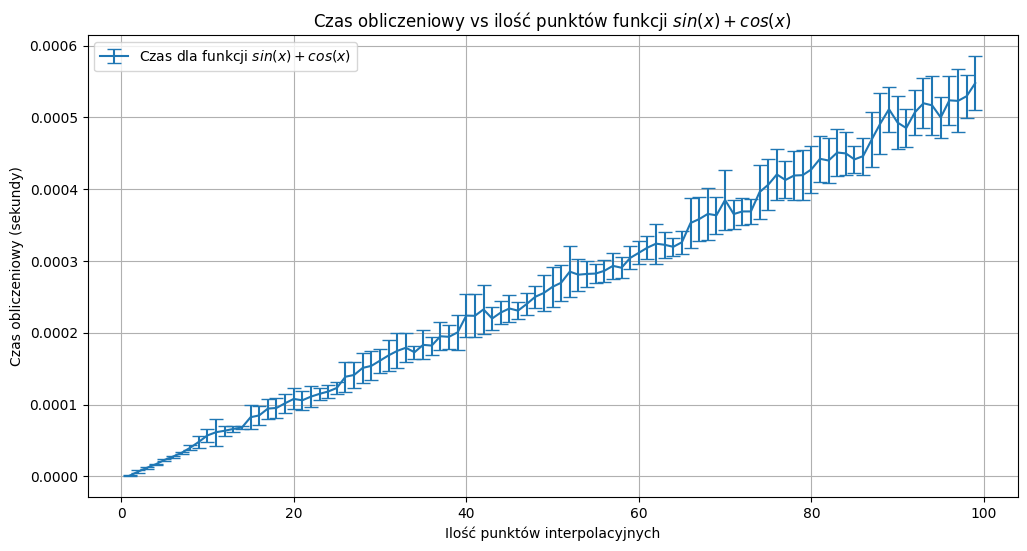
\includegraphics[width=\textwidth]{wykresy/zadanie 2/czas_tryg.png}
\end{minipage}

% wielomian 3 rzędu
\textbf{Wyniki dla wielomianu trzeciego rzędu:}  
Najmniejszy błąd: \( 8.21 \times 10^{-14} \pm 1.31 \times 10^{-13} \)  
przy 9 punktach.  

\begin{minipage}{0.49\textwidth}
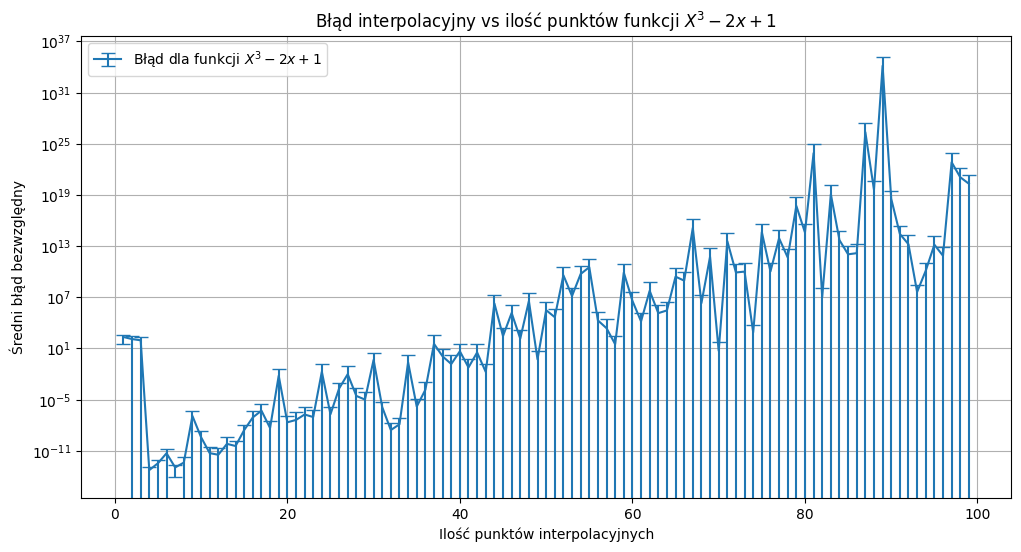
\includegraphics[width=\textwidth]{wykresy/zadanie 2/blad_wiel.png}
\end{minipage}
\begin{minipage}{0.49\textwidth}
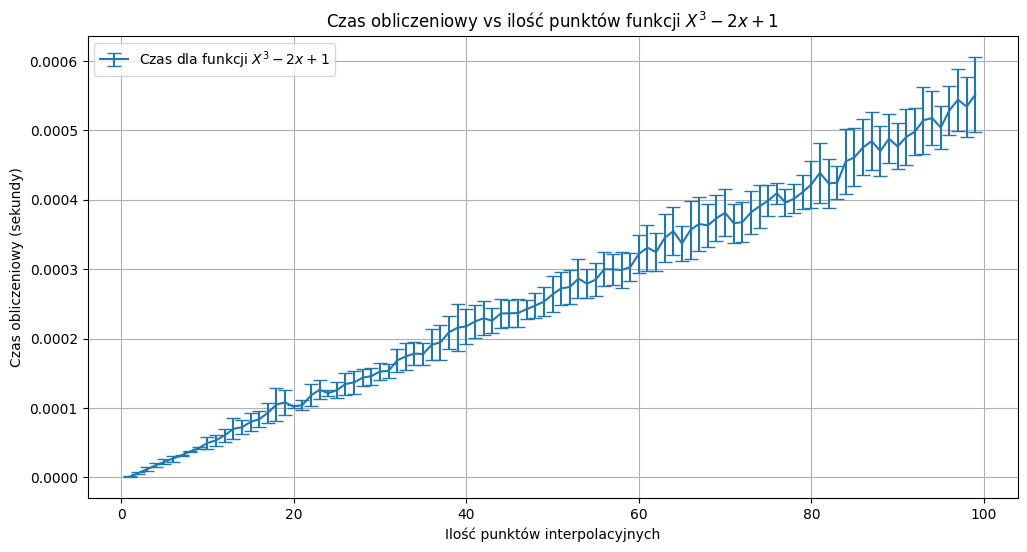
\includegraphics[width=\textwidth]{wykresy/zadanie 2/czas_wiel.png}
\end{minipage}

% exponenta
\textbf{Wyniki dla funkcji exp:}  
Najmniejszy błąd: \( 2.00 \times 10^{-9} \pm 1.25 \times 10^{-8} \)  
przy 26 punktach. 

\begin{minipage}{0.49\textwidth}
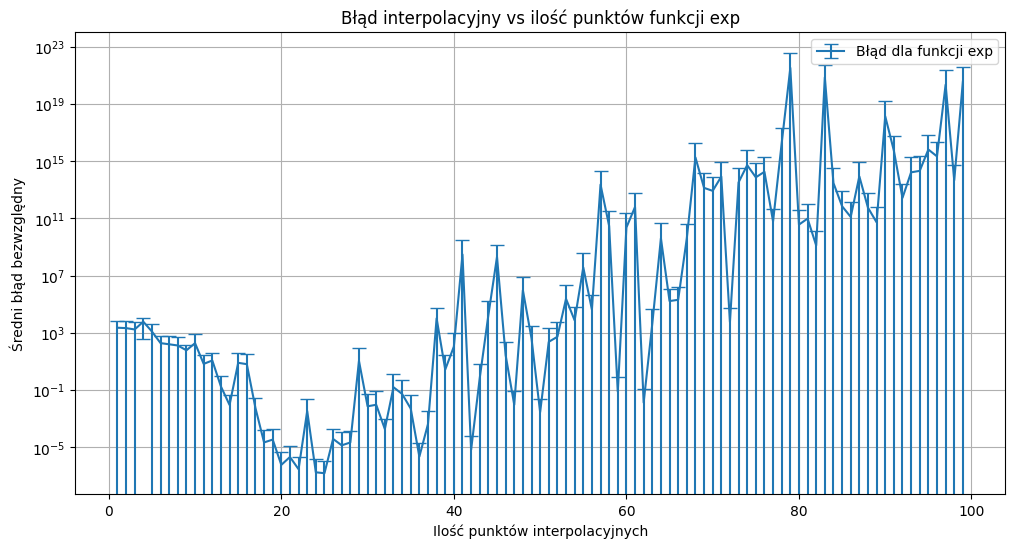
\includegraphics[width=\textwidth]{wykresy/zadanie 2/blad_exp.png}
\end{minipage}
\begin{minipage}{0.49\textwidth}
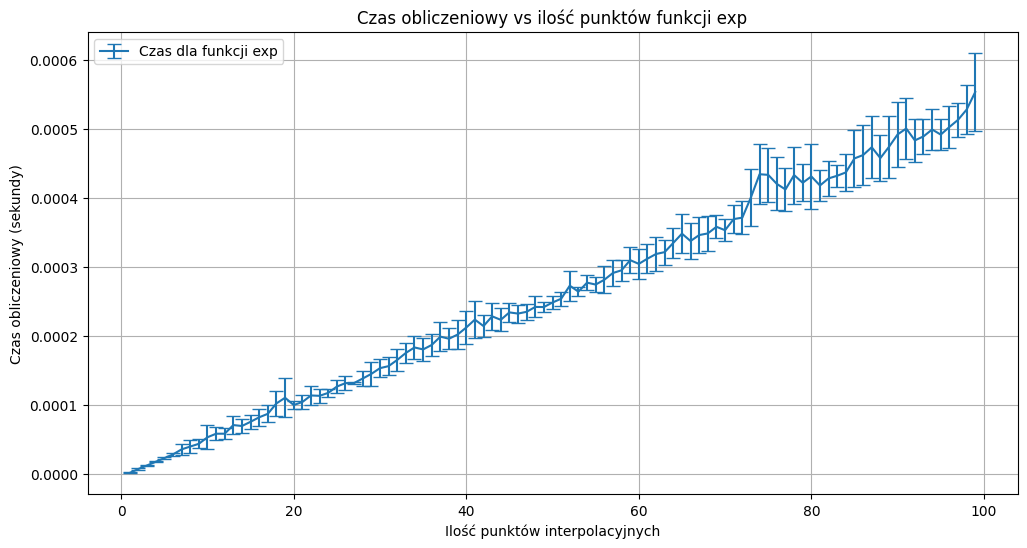
\includegraphics[width=\textwidth]{wykresy/zadanie 2/czas_exp.png}
\end{minipage}

% funkcja wymierna
\textbf{Wyniki dla funcji $\frac{1}{1 + x^2}$:}  
Najmniejszy błąd: \( 7.63 \times 10^{-12} \pm 3.28 \times 10^{-11} \)  
przy 28 punktach.

\begin{minipage}{0.49\textwidth}
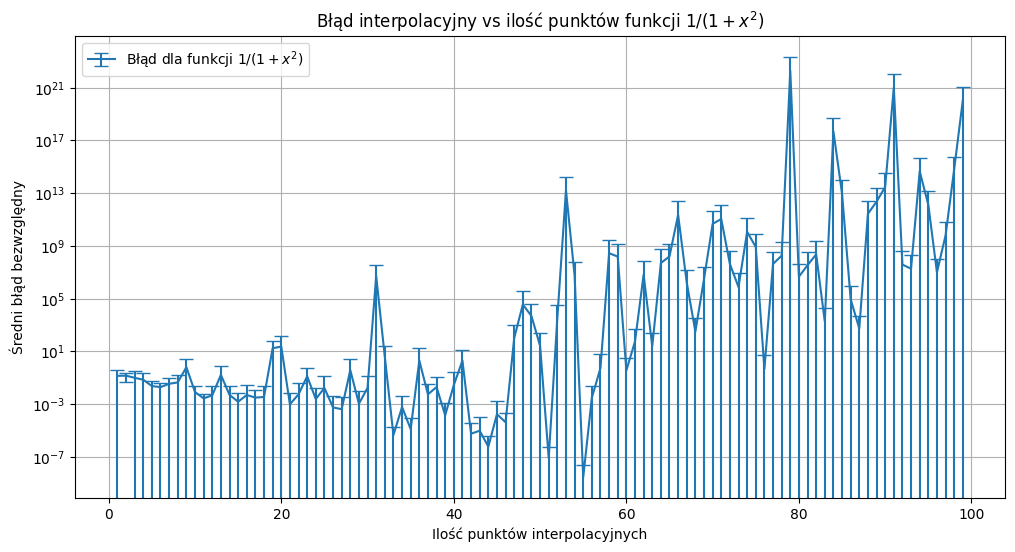
\includegraphics[width=\textwidth]{wykresy/zadanie 2/blad_wym.png}
\end{minipage}
\begin{minipage}{0.49\textwidth}
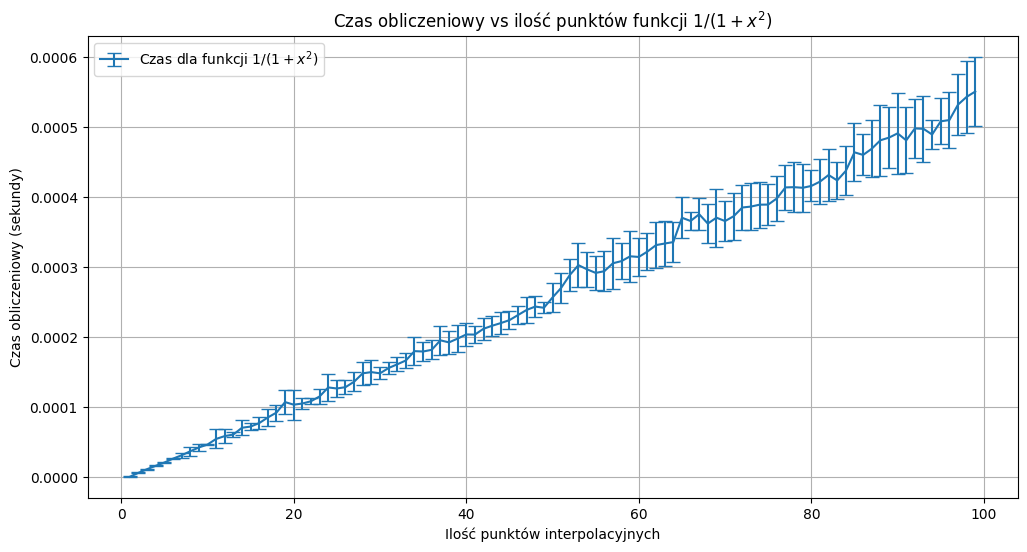
\includegraphics[width=\textwidth]{wykresy/zadanie 2/czas_wym.png}
\end{minipage}
\end{center}

\textbf{Wnioski:}
\begin{itemize}
    \item \textbf{Precyzja dla 10–20 punktów:} Przy wyborze od 10 do 20 punktów osiągano najlepsze wyniki pod względem dokładności, ponieważ przy większej liczbie punktów wzrastają błędy, głównie z powodu efektów numerycznych wynikających z dużych wartości przyrostów. Widzimy jednak duże odchylenie standardowe 
    \item \textbf{Czas obliczeń:} Czas wykonania algorytmu Neville'a był liniowy w zależności od liczby punktów, z bardzo małym współczynnikiem przyrostu. Wynika to z implementacji.
    \item \textbf{Różnice między funkcjami:} Największe błędy zaobserwowano w przypadku funkcji wykładniczej, co wynika z jej szybkiego wzrostu w przedziale \( D \). Najmniejsze błędy odnotowano dla wielomianu sześciennego, co jest zgodne z oczekiwaniami, gdyż metoda interpolacji wielomianowej jest idealna dla funkcji tego typu.
    \item \textbf{Odchylenie standardowe, błąd} Dziwne pokazywanie odchylenia standardowe jest spowodowane, przeskalowaniem wykresu. Głównie niesie informacje czy wyskakuje ono znacznie w górę. 
\end{itemize}

\newpage


% TODO zrobić tą tabele jeszce raz 
\section{Zadanie 3/4}

\subsection{Charakterystyka algorytmu Newtona}

Algorytm Newtona oparty na podzielonych różnicach jest techniką służącą do interpolacji funkcji. Jego główną zaletą jest efektywne obliczanie wartości wielomianu interpolacyjnego na podstawie zadanego zbioru punktów. Złożoność algorytmu wynosi \( O(n^2) \), co sprawia, że nadaje się on głównie do problemów z umiarkowaną liczbą danych wejściowych.

Podstawą algorytmu są podzielone różnice, które umożliwiają iteracyjne dodawanie kolejnych składników do wielomianu interpolacyjnego bez konieczności ponownego obliczania całości. W testach analizowano błędy w metryce Czebyszewa na 1000 punktach, próbe losowej $n$ i badano, jak dobrze dopasowanie odwzorowuje funkcję.

Eksperymenty przeprowadzono dla trzech funkcji:
\begin{itemize}
    \item Funkcja trygonometryczna: \( f(x) = \sin(x) + \cos(x) \),
    \item Funkcja wymierna: \( f(x) = \frac{1}{1 + x^2} \),
    \item Funkcja nieciągła: \( f(x) = \lfloor x \rfloor \).
\end{itemize}

\subsection{Wyniki i wnioski}

\begin{center}
% Wykres błędów dla funkcji
\textbf{Wyniki dla funkcji \( \sin(x) + \cos(x) \):}  
Minimalny błąd: \( 9.63 \times 10^{-10} \)  
Osiągnięty dla 33 punktów.  
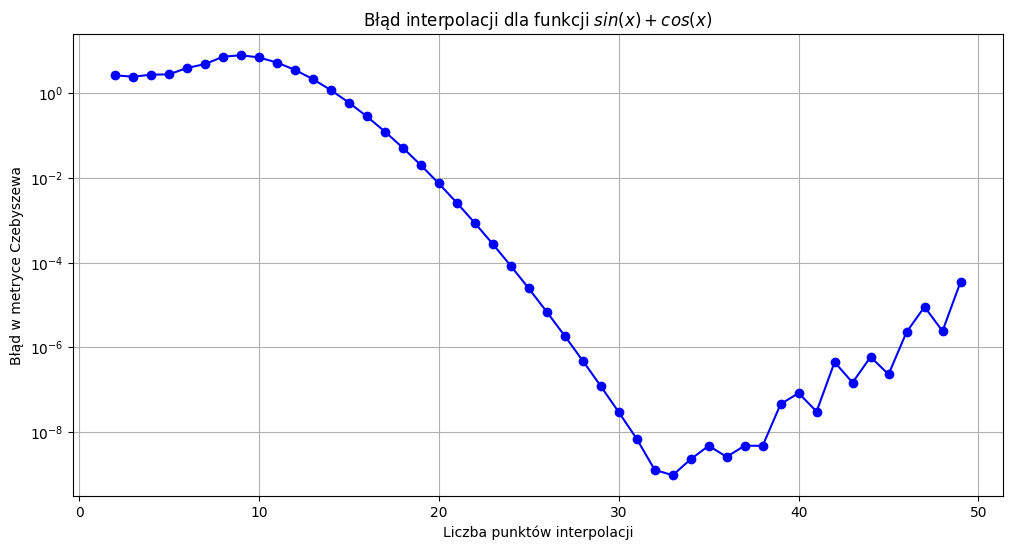
\includegraphics[width=0.8\textwidth]{wykresy/zadanie 3/tryg_blad.png}
\end{center}

\begin{minipage}{0.49\textwidth}
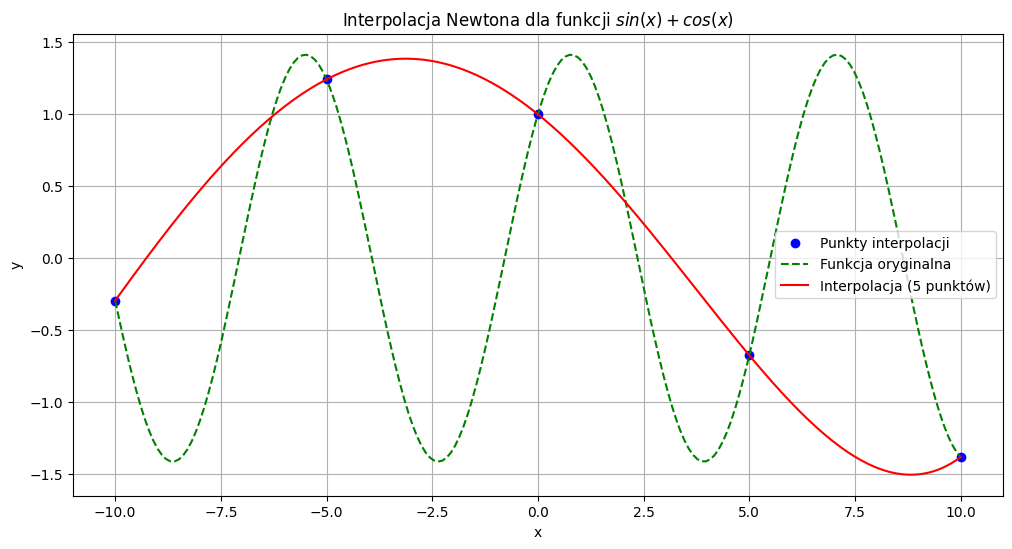
\includegraphics[width=\textwidth]{wykresy/zadanie 3/tryg_5.png}
\end{minipage}
\begin{minipage}{0.49\textwidth}
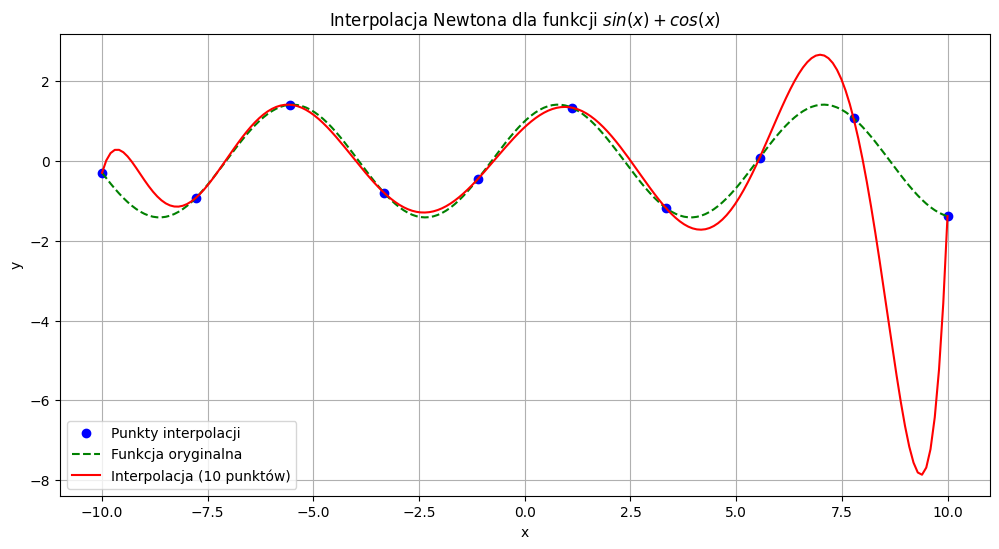
\includegraphics[width=\textwidth]{wykresy/zadanie 3/tryg_10.png}
\end{minipage}

\begin{minipage}{0.49\textwidth}
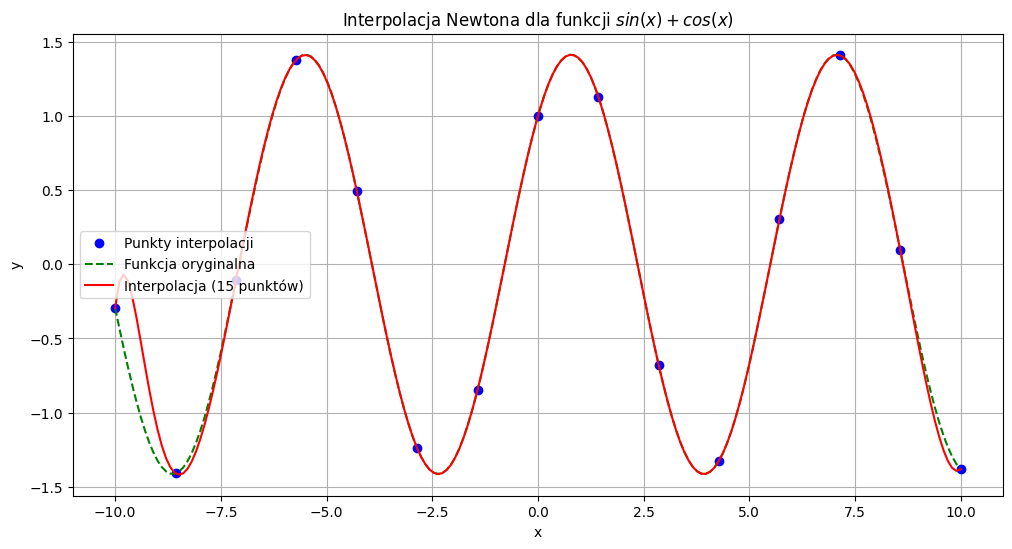
\includegraphics[width=\textwidth]{wykresy/zadanie 3/tryg_15.png}
\end{minipage}
\begin{minipage}{0.49\textwidth}
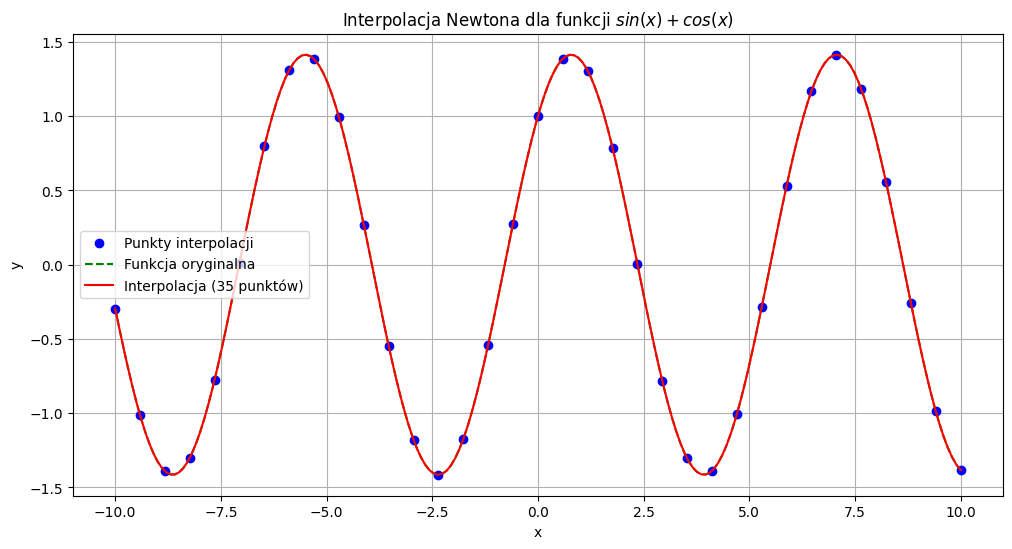
\includegraphics[width=\textwidth]{wykresy/zadanie 3/tryg_35.png}
\end{minipage}

\begin{center}
% Wykres błędów dla funkcji wymiernej
\textbf{Wyniki dla funkcji \( \frac{1}{1 + x^2} \):}  
Minimalny błąd: \( 4.78 \times 10^{-1} \)  
Osiągnięty dla 10 punktów.  
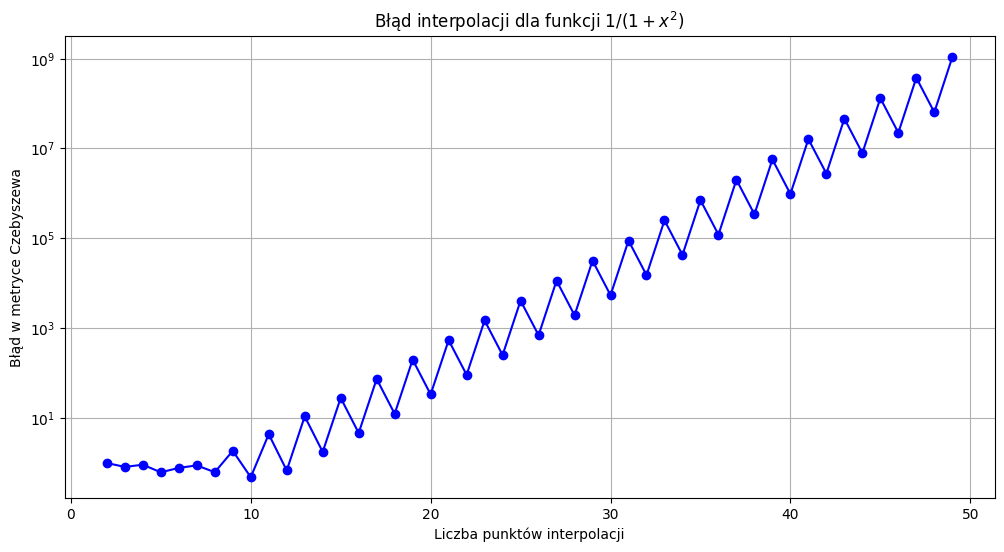
\includegraphics[width=0.8\textwidth]{wykresy/zadanie 3/wym_blad.png}
\end{center}

\begin{minipage}{0.49\textwidth}
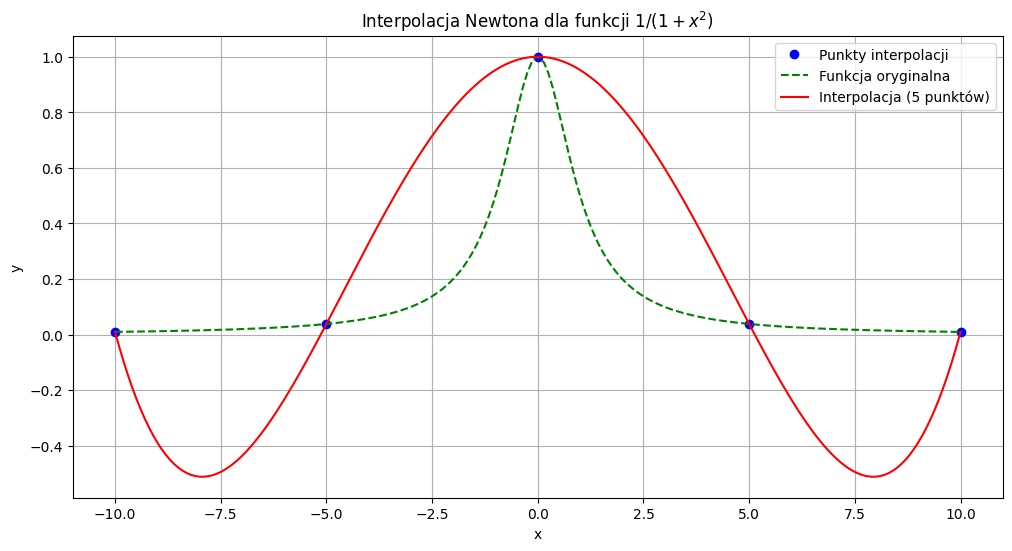
\includegraphics[width=\textwidth]{wykresy/zadanie 3/wym_5.png}
\end{minipage}
\begin{minipage}{0.49\textwidth}
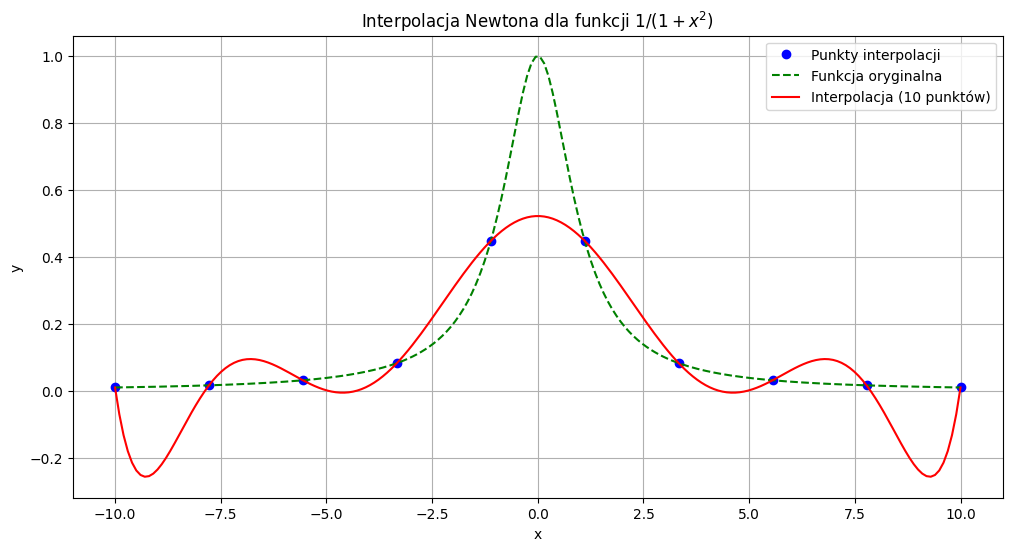
\includegraphics[width=\textwidth]{wykresy/zadanie 3/wym_10.png}
\end{minipage}

\begin{minipage}{0.49\textwidth}
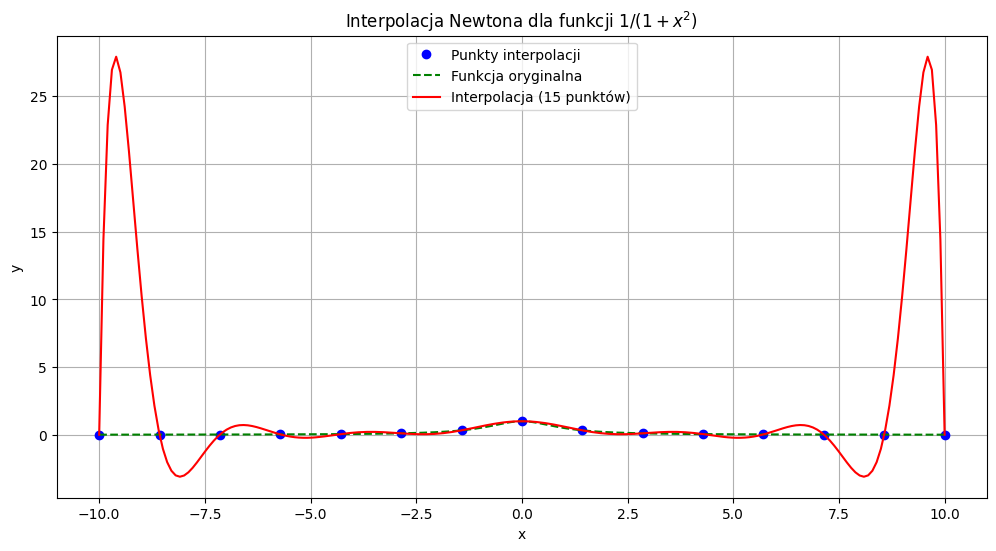
\includegraphics[width=\textwidth]{wykresy/zadanie 3/wym_15.png}
\end{minipage}
\begin{minipage}{0.49\textwidth}
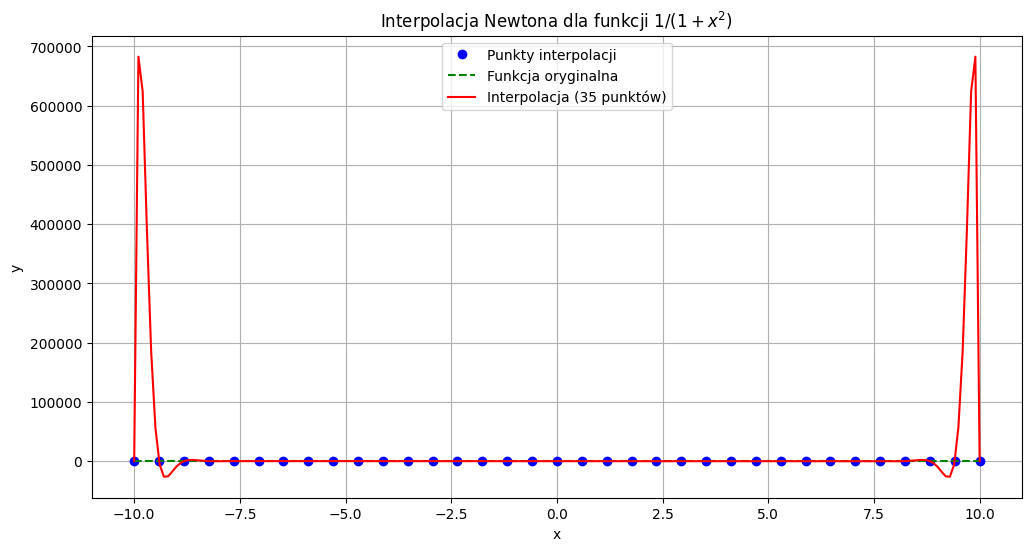
\includegraphics[width=\textwidth]{wykresy/zadanie 3/wym_35.png}
\end{minipage}

\begin{center}
% Wykres błędów dla funkcji podłoga
\textbf{Wyniki dla funkcji \( \lfloor x \rfloor \):}  
Minimalny błąd: \( 9.32 \times 10^{-1} \)  
Osiągnięty dla 20 punktów.  
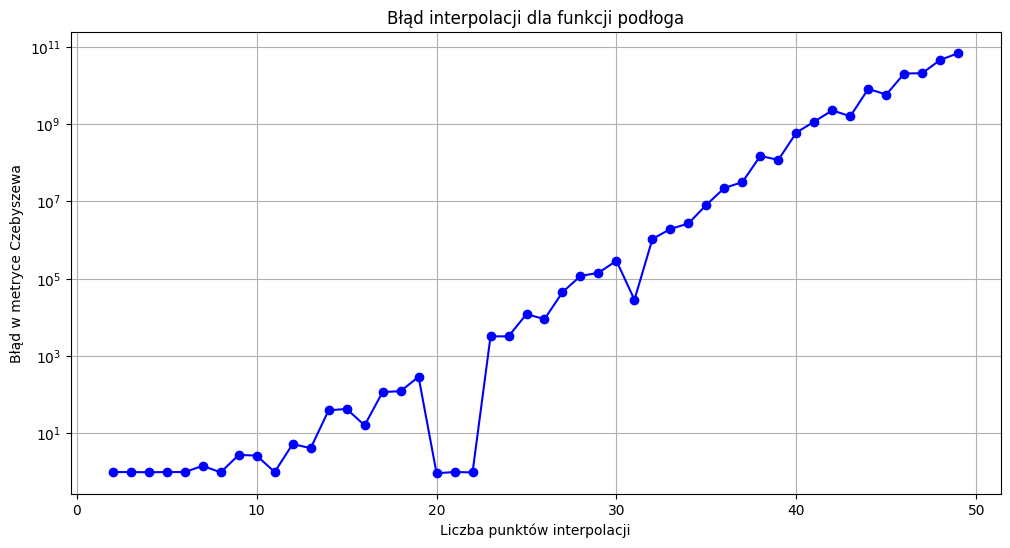
\includegraphics[width=0.8\textwidth]{wykresy/zadanie 3/floor_blad.png}
\end{center}

\begin{minipage}{0.49\textwidth}
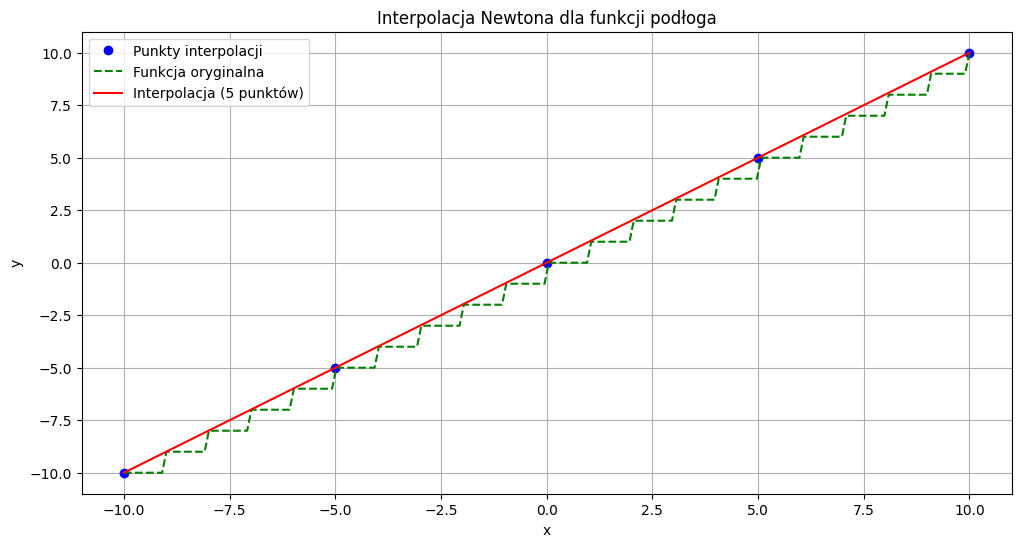
\includegraphics[width=\textwidth]{wykresy/zadanie 3/floor_5.png}
\end{minipage}
\begin{minipage}{0.49\textwidth}
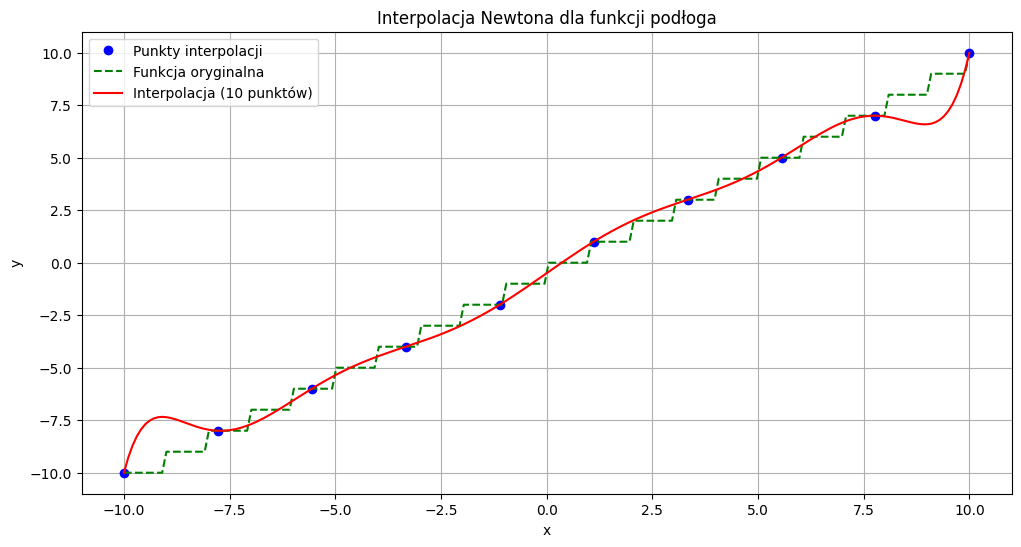
\includegraphics[width=\textwidth]{wykresy/zadanie 3/floor_10.png}
\end{minipage}

\begin{minipage}{0.49\textwidth}
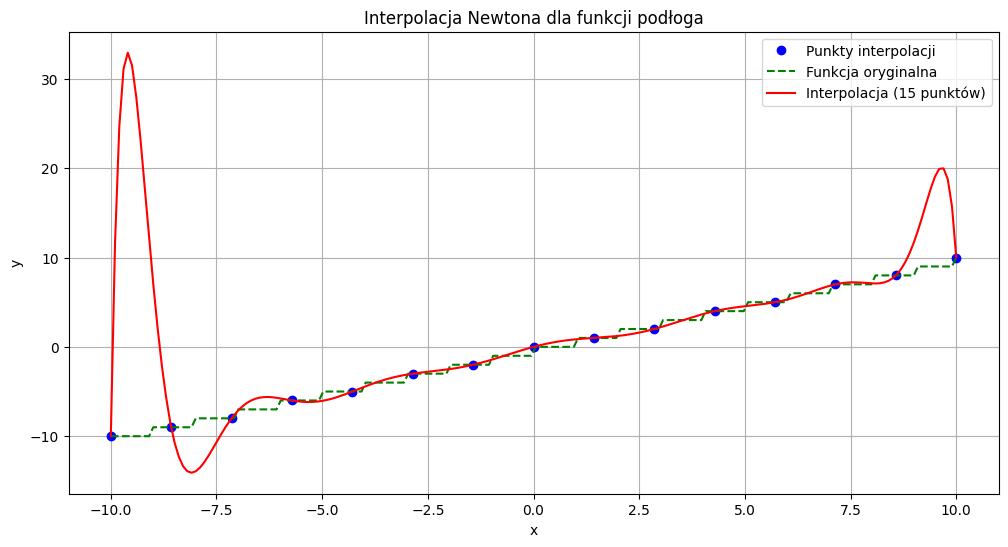
\includegraphics[width=\textwidth]{wykresy/zadanie 3/floor_15.png}
\end{minipage}
\begin{minipage}{0.49\textwidth}
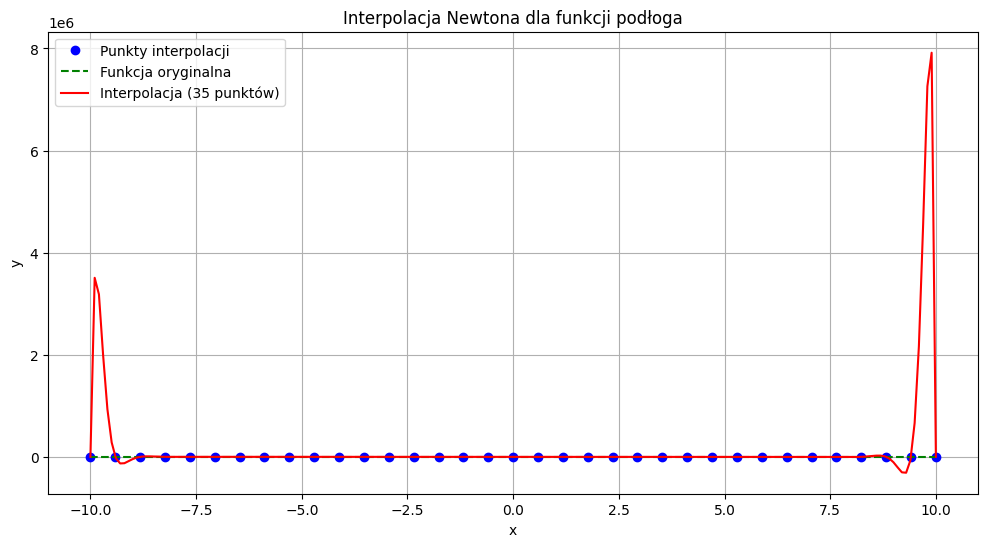
\includegraphics[width=\textwidth]{wykresy/zadanie 3/floor_35.png}
\end{minipage}

\textbf{Wnioski:}
\begin{itemize}
    \item \textbf{Efektywność przy umiarkowanej liczbie punktów:} Dodawanie dużej liczby punktów interpolacyjnych niekoniecznie poprawia wyniki. Wręcz przeciwnie, prowadzi to do większych błędów, ponieważ algorytm próbuje dopasować wielomian, co wymaga nagłych wzrostów wartości funkcji.
    \item \textbf{Trudności z funkcjami nieciągłymi:} W przypadku funkcji nieciągłych, takich jak \( \lfloor x \rfloor \), uzyskiwane błędy są znacznie większe, co wynika z problemów z dopasowaniem ciągłego wielomianu do nieciągłości.
    \item \textbf{Funkcje jednostajnie ciągłe:} Funkcje jednostajnie ciągłe, takie jak trygonometryczna i wymierna, pozwalają na uzyskanie lepszych wyników, choć nawet w tych przypadkach obserwowane są pewne ograniczenia dokładności.
    \item przy funkcjach mają wiele ekstermów widzimy charakterystyczny skoki, które wynikają z częstych zmian tempa przyrostu. 
\end{itemize}

\newpage



\section{Zadanie 5}

\subsection{Charakterystyka algorytmu Clenshawa}

Algorytm Clenshawa to efektywna metoda obliczania wartości wielomianu w postaci Czebyszewa przy złożoności \( O(n) \). W porównaniu ze standardowym sposobem wyznaczania wartości wielomianów, algorytm ten jest zoptymalizowany do przetwarzania ich w postaci rekurencyjnej, co prowadzi do znacznego przyspieszenia obliczeń.

W ramach eksperymentu porównano szybkość działania algorytmu Clenshawa z klasycznym sposobem obliczania wielomianów Czebyszewa. Wyniki przedstawiono na wykresie, który uwzględnia średni czas wykonania dla obu metod. Ustawienia jak w zadaniu 1.

\subsection{Wyniki i wnioski}

\begin{center}
% Wykres czasu porównania Clenshawa i metody standardowej
\textbf{Średni czas dla metody Clenshawa:} \( 0.000578 \pm 0.000324 \)  
\textbf{Średni czas dla metody standardowej:} \( 0.000692 \pm 0.000393 \)  
\textbf{Przyspieszenie:} \( 1.20 \times \pm 0.03 \times \)
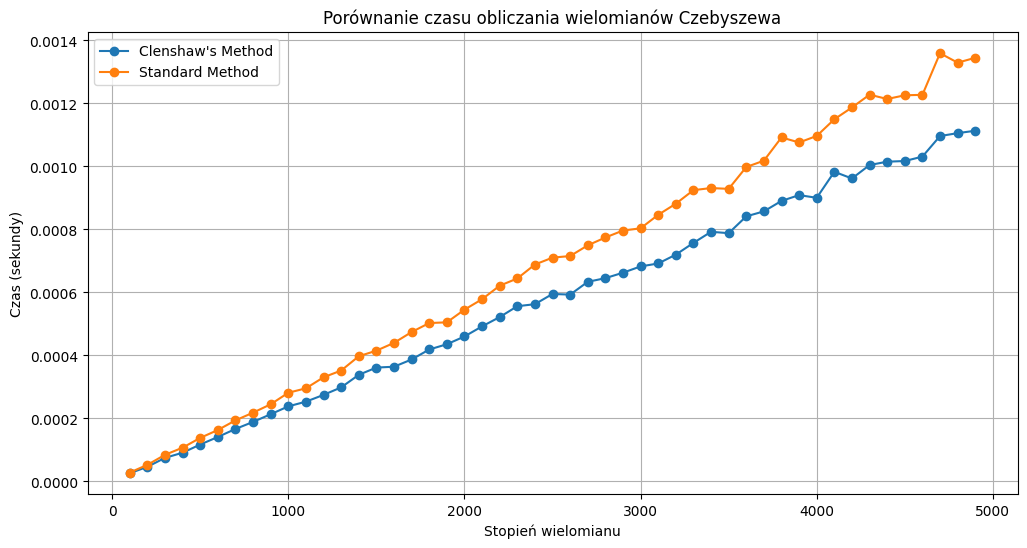
\includegraphics[width=\textwidth]{wykresy/zadanie 4/czebyszew_5000.png}
\end{center}

\textbf{Wnioski:}
\begin{itemize}
    \item \textbf{Szybkość metody Clenshawa:} Algorytm Clenshawa wykazuje wyraźną przewagę nad standardową metodą liczenia wielomianów Czebyszewa, osiągając średnio 1.20x szybsze wykonanie.
    \item \textbf{Porównanie z Hornerem:} Metoda Clenshawa jest bliska optymalnemu czasowi obliczeń znanemu z algorytmu Hornera, który jest specjalnym przypadkiem dla wielomianów Czebyszewa.
    \item \textbf{Stabilność czasów:} W odróżnieniu od algorytmu Hornera, metoda Clenshawa nie wykazuje wahań w czasie wykonania, co świadczy o jej większej stabilności numerycznej.
\end{itemize}

\newpage

\section{Zadanie 6}

\subsection{Charakterystyka algorytmu interpolacji trygonometrycznej}

Algorytm interpolacji trygonometrycznej pozwala na aproksymację funkcji okresowych za pomocą wielomianów trygonometrycznych. Złożoność tego algorytmu wynosi \( O(n \cdot m) \), gdzie \( n \) to liczba punktów interpolacyjnych (\( n = 2m \)), a \( m \) jest liczbą współczynników w wielomianie. W szczególności algorytm korzysta z okresowych wartości funkcji w równomiernie rozłożonych węzłach, co pozwala na wyznaczenie współczynników aproksymacji trygonometrycznej. 

W ramach eksperymentu zbadano, jak zmienia się błąd interpolacji w zależności od liczby punktów \( m \) oraz jak dobrze algorytm odtwarza wybrane funkcje (ciągłe i nieciągłe). Wyniki zaprezentowano na wykresach. Ustawienia jak w zadaniu 3/4.


\subsection{Wyniki i wnioski}

\begin{center}
% Wykres błędów dla funkcji
\textbf{Wyniki dla funkcji \( \sin(x) + \cos(x) \):}  
Minimalny błąd: \( 2.22e-16 \)  
Osiągnięty dla \( m = 3 \)  
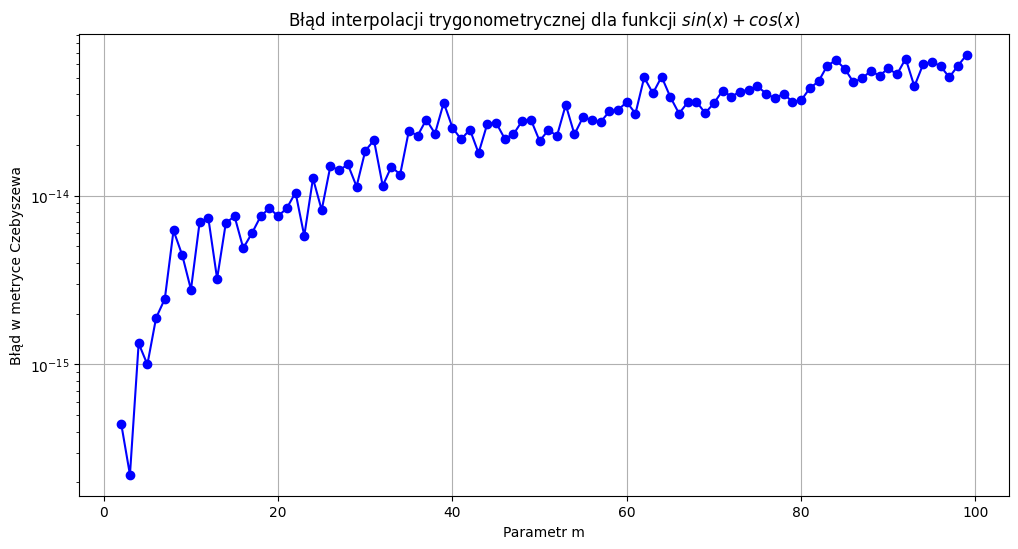
\includegraphics[width=0.8\textwidth]{wykresy/zadanie 5/tryg_blad.png}
\end{center}

\begin{minipage}{0.49\textwidth}
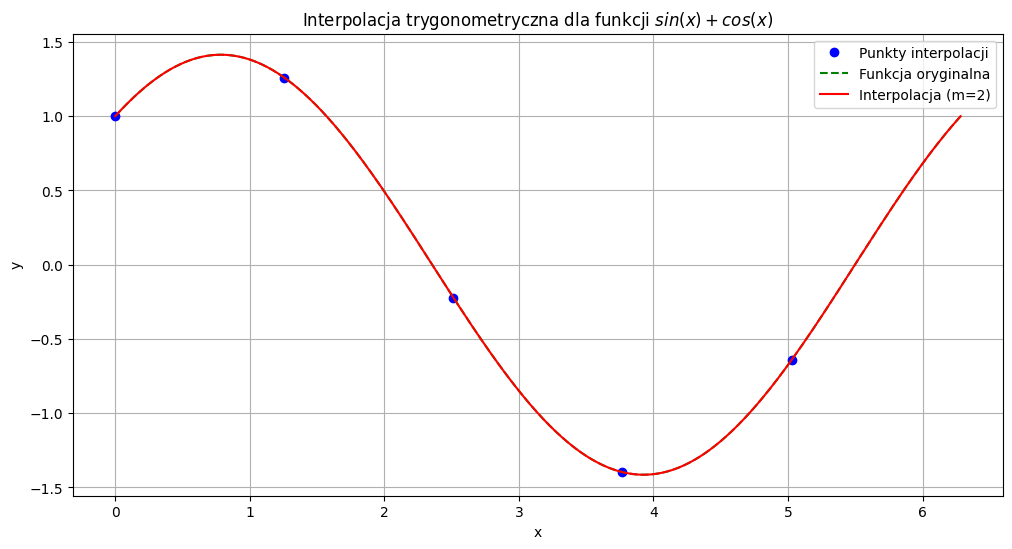
\includegraphics[width=\textwidth]{wykresy/zadanie 5/tryg_2.png}
\end{minipage}
\begin{minipage}{0.49\textwidth}
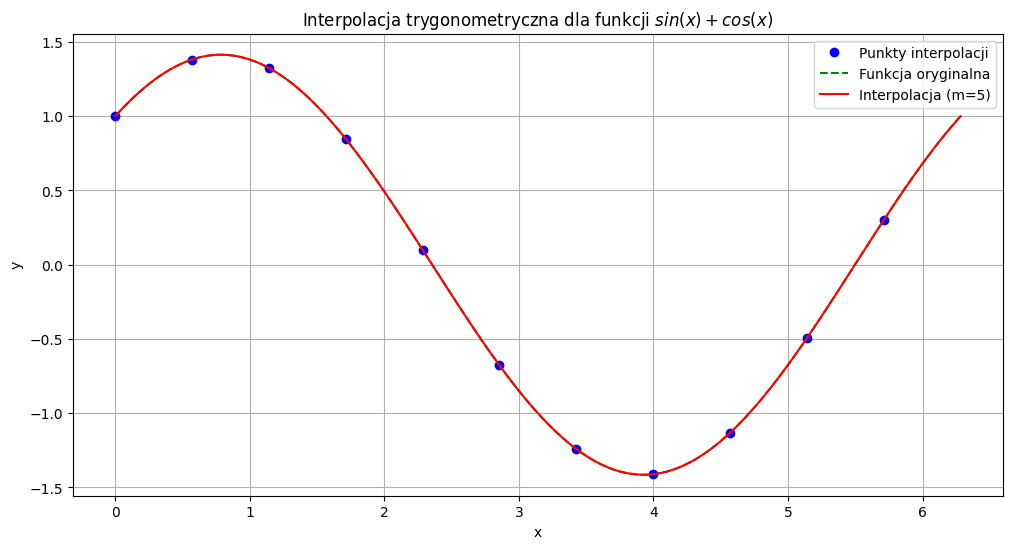
\includegraphics[width=\textwidth]{wykresy/zadanie 5/tryg_5.png}
\end{minipage}

\begin{minipage}{0.49\textwidth}
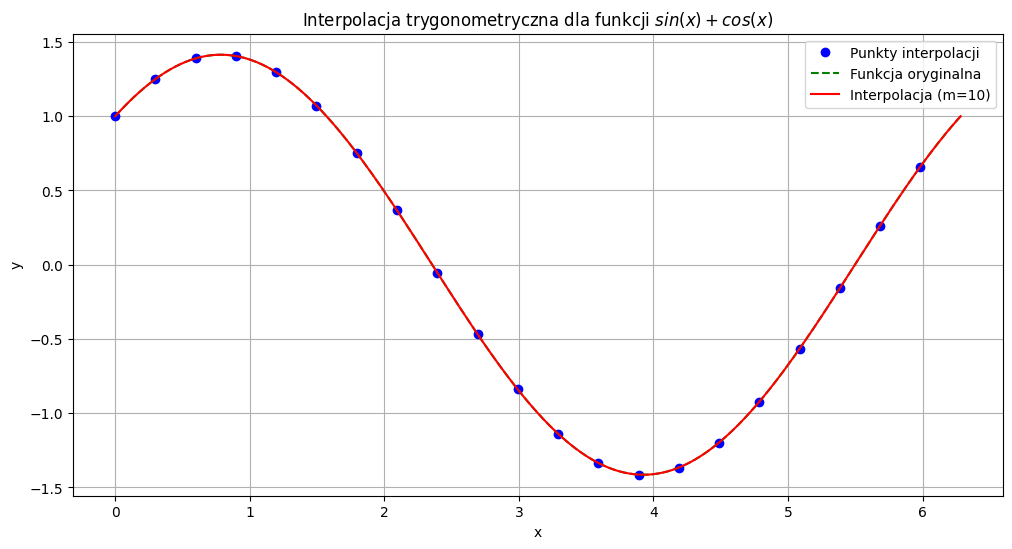
\includegraphics[width=\textwidth]{wykresy/zadanie 5/tryg_10.png}
\end{minipage}
\begin{minipage}{0.49\textwidth}
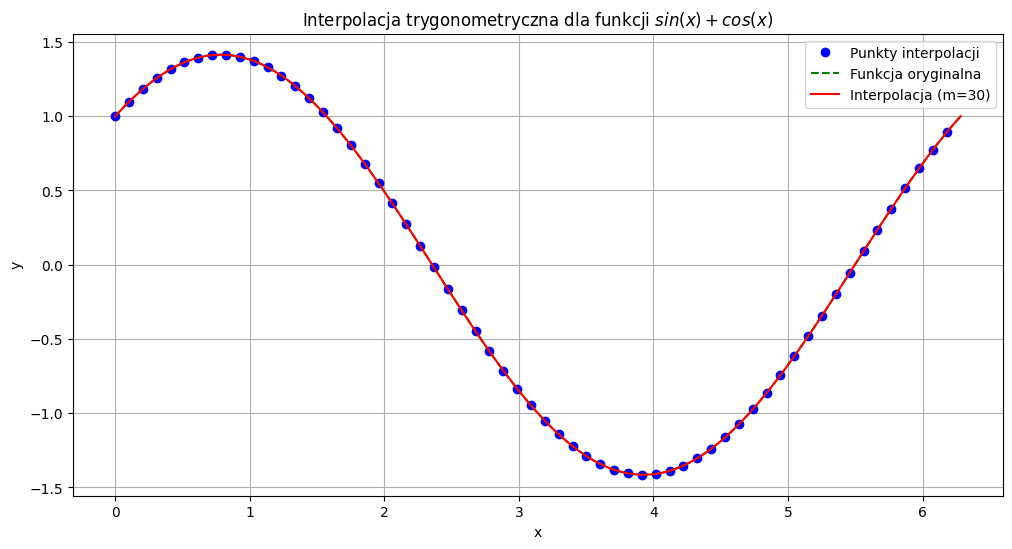
\includegraphics[width=\textwidth]{wykresy/zadanie 5/tryg_30.png}
\end{minipage}

\begin{center}
\textbf{Wyniki dla funkcji \( \frac{1}{1+x^2} \):}  
Minimalny błąd: \( 9.75e-01 \)  
Osiągnięty dla \( m = 89 \)  
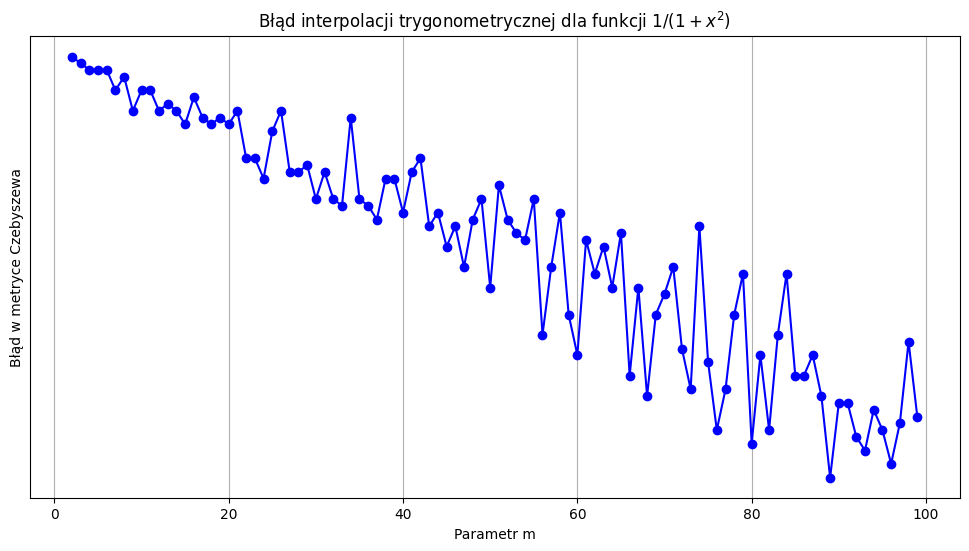
\includegraphics[width=0.8\textwidth]{wykresy/zadanie 5/wym_blad.png}
\end{center}

\begin{minipage}{0.49\textwidth}
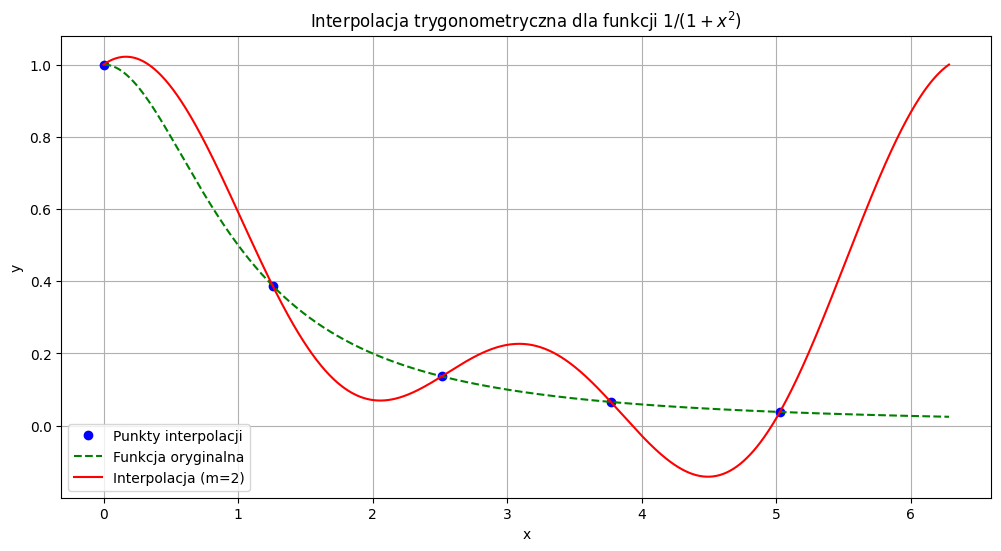
\includegraphics[width=\textwidth]{wykresy/zadanie 5/wym_2.png}
\end{minipage}
\begin{minipage}{0.49\textwidth}
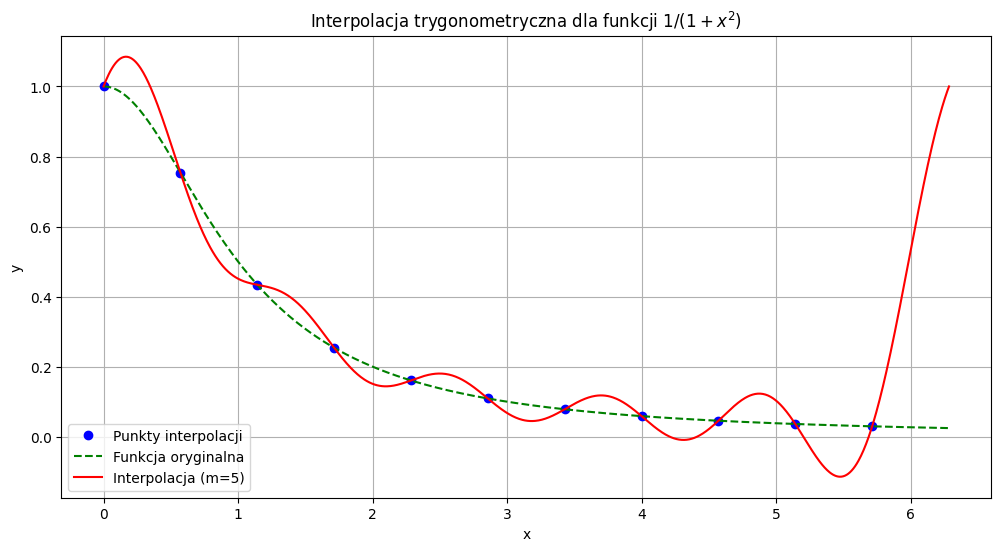
\includegraphics[width=\textwidth]{wykresy/zadanie 5/wym_5.png}
\end{minipage}

\begin{minipage}{0.49\textwidth}
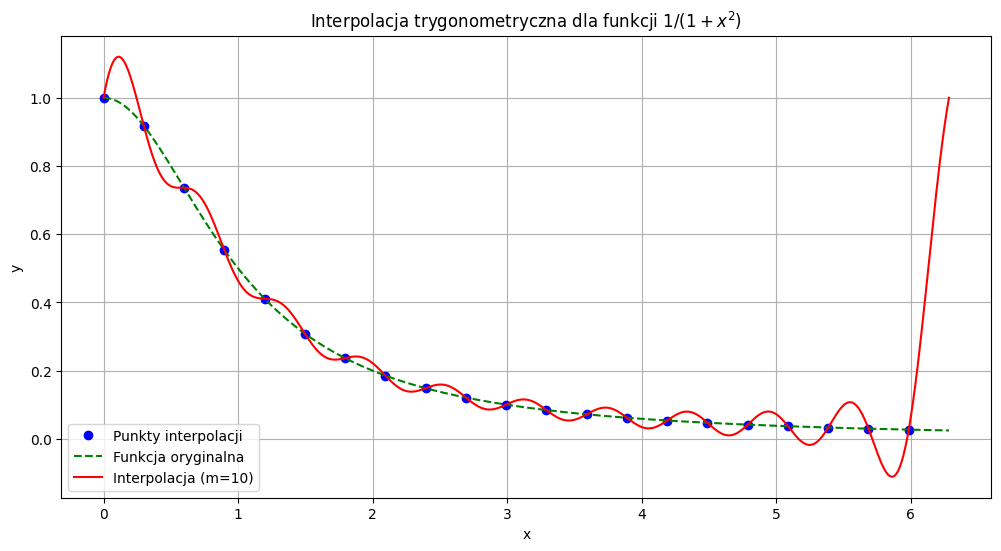
\includegraphics[width=\textwidth]{wykresy/zadanie 5/wym_10.png}
\end{minipage}
\begin{minipage}{0.49\textwidth}
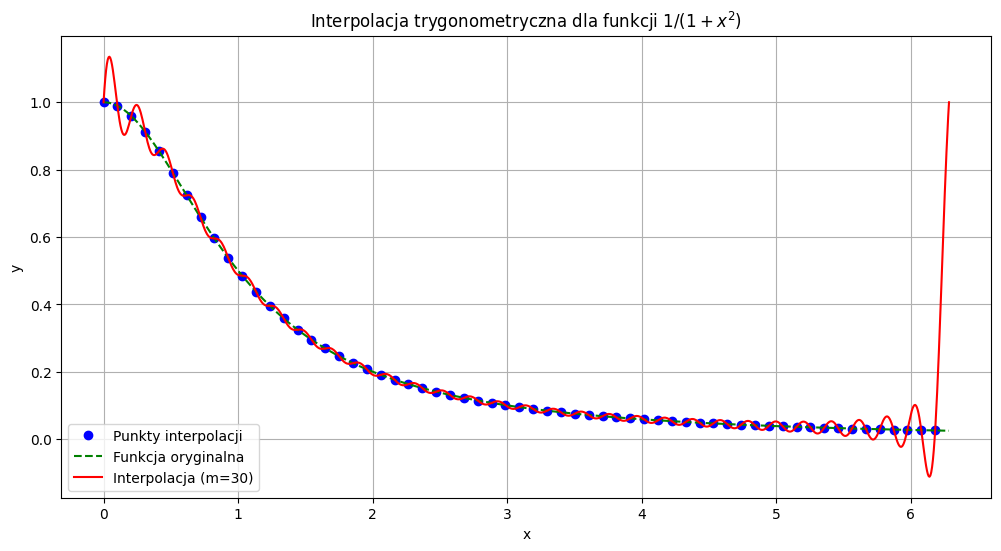
\includegraphics[width=\textwidth]{wykresy/zadanie 5/wym_30.png}
\end{minipage}

\begin{center}
% Wykres błędów dla funkcji podłoga
\textbf{Wyniki dla funkcji podłoga:}  
Minimalny błąd: \( 6.00e+00 \)  
Osiągnięty dla \( m = 99 \)  
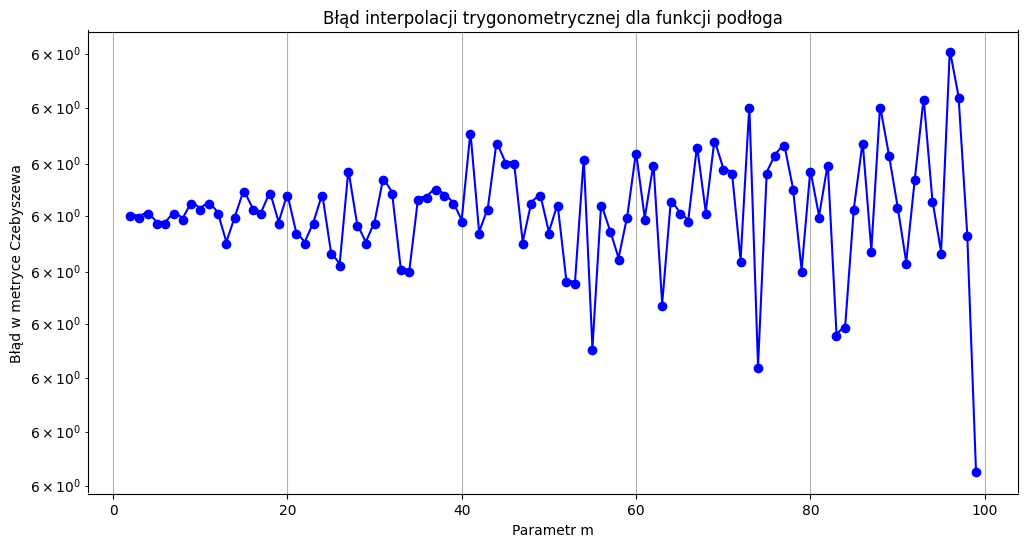
\includegraphics[width=0.8\textwidth]{wykresy/zadanie 5/floor_blad.png}
\end{center}

\begin{minipage}{0.49\textwidth}
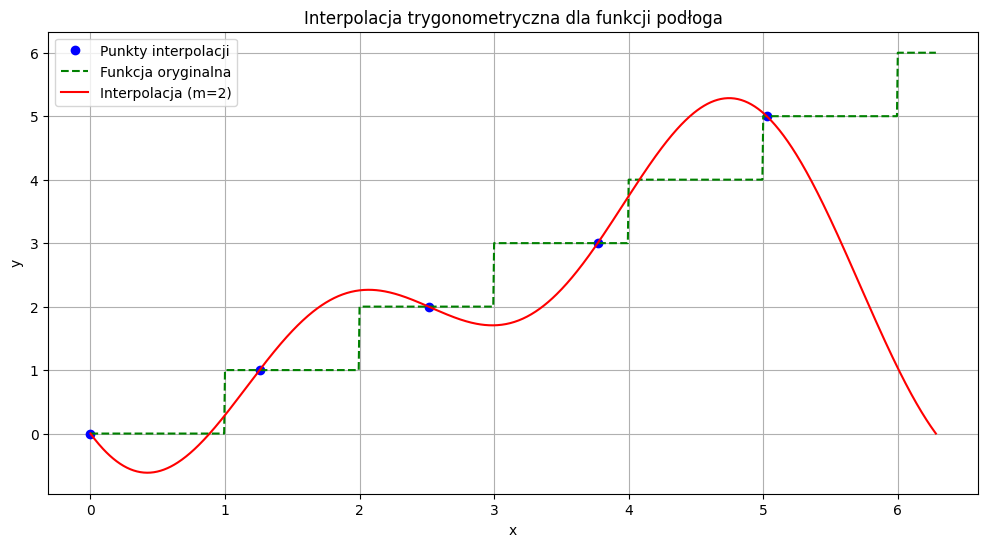
\includegraphics[width=\textwidth]{wykresy/zadanie 5/floor_2.png}
\end{minipage}
\begin{minipage}{0.49\textwidth}
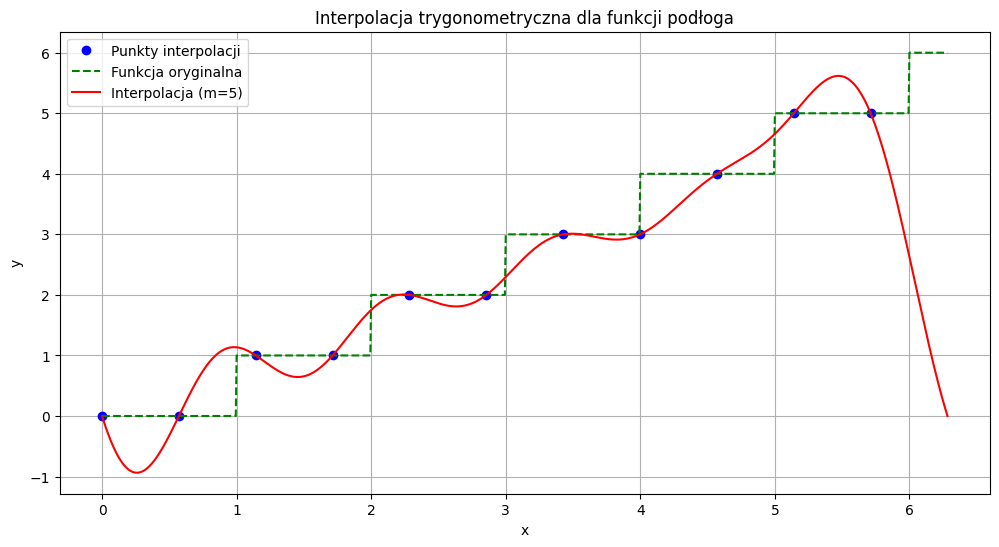
\includegraphics[width=\textwidth]{wykresy/zadanie 5/floor_5.png}
\end{minipage}

\begin{minipage}{0.49\textwidth}
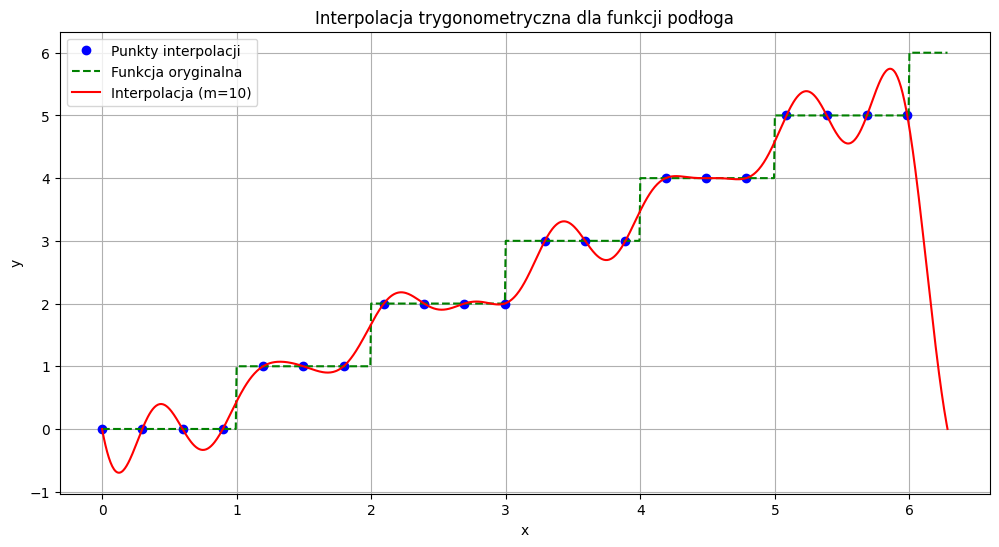
\includegraphics[width=\textwidth]{wykresy/zadanie 5/floor_10.png}
\end{minipage}
\begin{minipage}{0.49\textwidth}
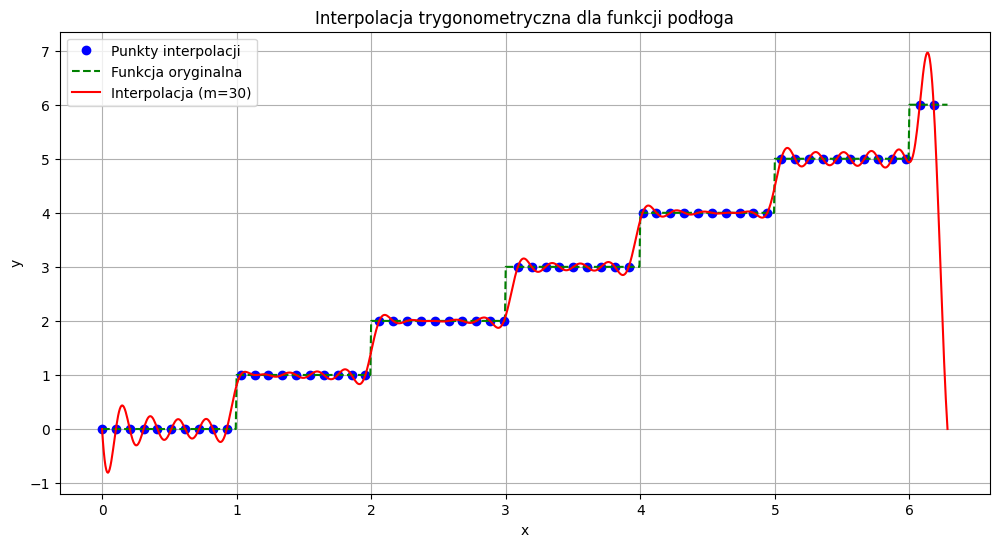
\includegraphics[width=\textwidth]{wykresy/zadanie 5/floor_30.png}
\end{minipage}

\textbf{Wnioski:}
\begin{itemize}
    \item \textbf{Dokładność:} Algorytm interpolacji trygonometrycznej charakteryzuje się bardzo małymi błędami dla funkcji okresowych, takich jak \( \sin(x) + \cos(x) \). 
    \item \textbf{Interpolacja funkcji nieciągłych:} Pomimo swojej specyfiki, algorytm pozwala na interpolację funkcji nieciągłych (np. funkcji podłoga), choć błąd w tych przypadkach jest znacznie większy.
    \item \textbf{Odchylenia na końcach:} Wahania na końcu wykresów błędu wynikają z niedoskonałości implementacji, co można skorygować. W teorii, metoda powinna dawać wyniki zgodne z oczekiwaniami.
    \item \textbf{Uniwersalność:} Dzięki możliwości skalowania dziedziny do \( [0, 2\pi] \), metoda ma szerokie zastosowania i może być wykorzystywana do analizy wielu rodzajów funkcji.
\end{itemize}





% propozycje: 
% moment stopu, gdy, absolutny błąd bezwzględny, jest taki sam jak poprzedni


% \bibliographystyle{abbrv}
% \bibliography{references}  % need to put bibtex references in references.bib 
\end{document}